\chapter{\ChapterTitleRealizationAspects}
\label{sec:wybrane-aspekty-realizacji}

Ta sekcja pracy skupia się na opisaniu najważniejszych aspektów
opracowanej aplikacji.
Jej celem jest szczegółowe opisanie wybranych
komponentów oraz przedstawienie czynników, które są najistotniejsze do
funkcjonowania całości systemu. Dodatkowo skoncentruje
się na prezentacji skutecznych rozwiązań dla wykrytych problemów.

\section{Podział tworzonego systemu}

\begin{figure}[!]
  \centering
  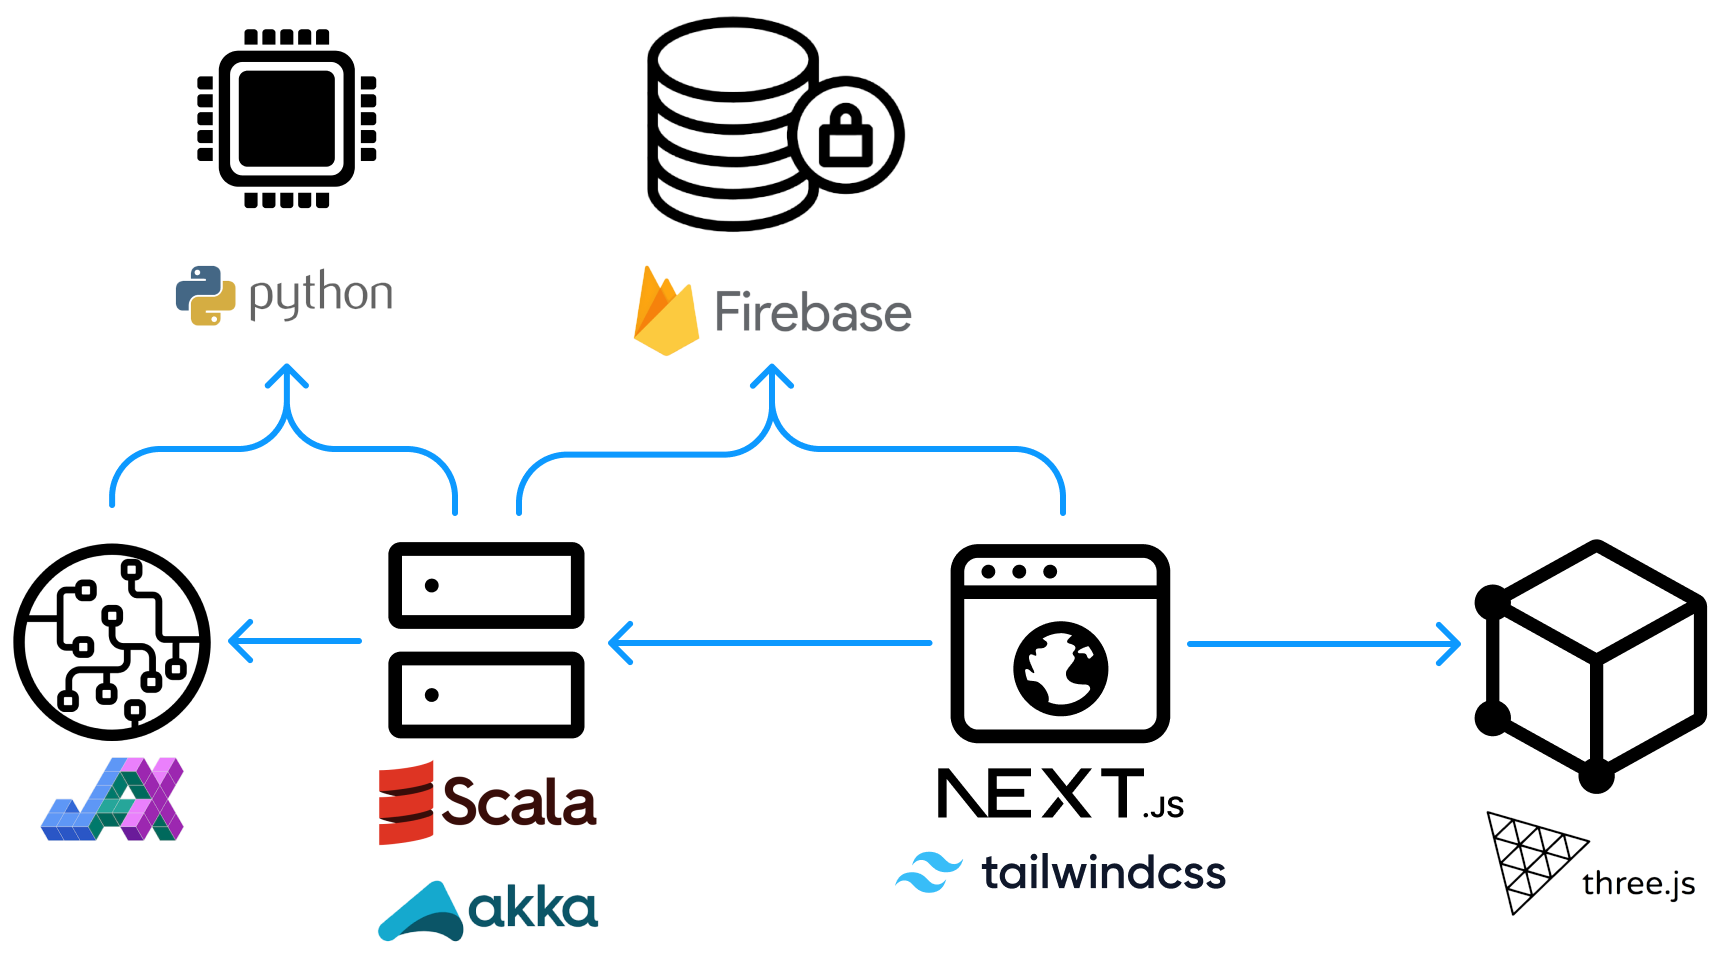
\includegraphics[width=\textwidth]{img/schematy/schemat_systemu.png}
  \caption{Schemat podziału i~zależności elementów systemu wraz z~wykorzystywanymi przez nie technologiami.}
  \label{fig:akka-highlevel}
\end{figure}

Aby usprawnić pracę nad produktem, podzieliliśmy system na osobne
fragmenty. Każdy z~nich odpowiedzialny był za inną jego część.
Podczas pracy nad osobnymi elementami ważne było, aby mogły się one
ze sobą komunikować. W~tym celu w~trakcie projektowania
całości systemu zostały stworzone odpowiednie schematy definiujące
odpowiedzialność każdego elementu, jak i~w~jaki sposób ma się odbywać
dialog pomiędzy nimi. Opisane w~nich też zostały abstrakcyjne
obiekty dzielące odpowiedzialność za przechowywanie informacji
potrzebnych do działania systemu. Pozwoliło to na zdefiniowanie,
za co ma odpowiadać każdy z~elementów.

Podzielono system na następujące elementy:
\begin{itemize}
  \item Bridge Core -- główna logika gry w~brydża; stworzona
        w~języku Python,

  \item Wirtualny asystent -- biblioteka pozwalająca na uczestniczenie
        w~brydzu jako gracz; stworzony w~środowisku JAX.

  \item Aplikacja webowa -- główny interfejs dla użytkowników,
        aby móc rozgrywać grę; stworzone przy zastosowaniu
        frameworków Next.js i~Tailwind.css w~językach HTML, \mbox{Javascript}
        oraz CSS,

  \item Serwer gry -- centralny serwer, którego zadaniem jest
        łączenie graczy do sesji, przeprowadzanie gier i~zarządzaie
        w~nich asystentem; stworzony przy użyciu języku Scala
        \mbox{i~frameworku} Akka,

  \item Bridge Engine -- interfejs gry brydża; stworzony
        z~użyciem frameworka Three.js i~języku Javascript,

  \item Google Firebase -- osobny system Google'a, który
        odpowiada za zarządzanie i~uwierzytelnianie użytkowników.
\end{itemize}

%%% TODO schemat abstrakcyjnego podziału systemu (sesja, lobby, sesja gry, uzytkwonicy, ai)

\FloatBarrier


\section{Architektura serwera}

\begin{figure}[!]
  \centering
  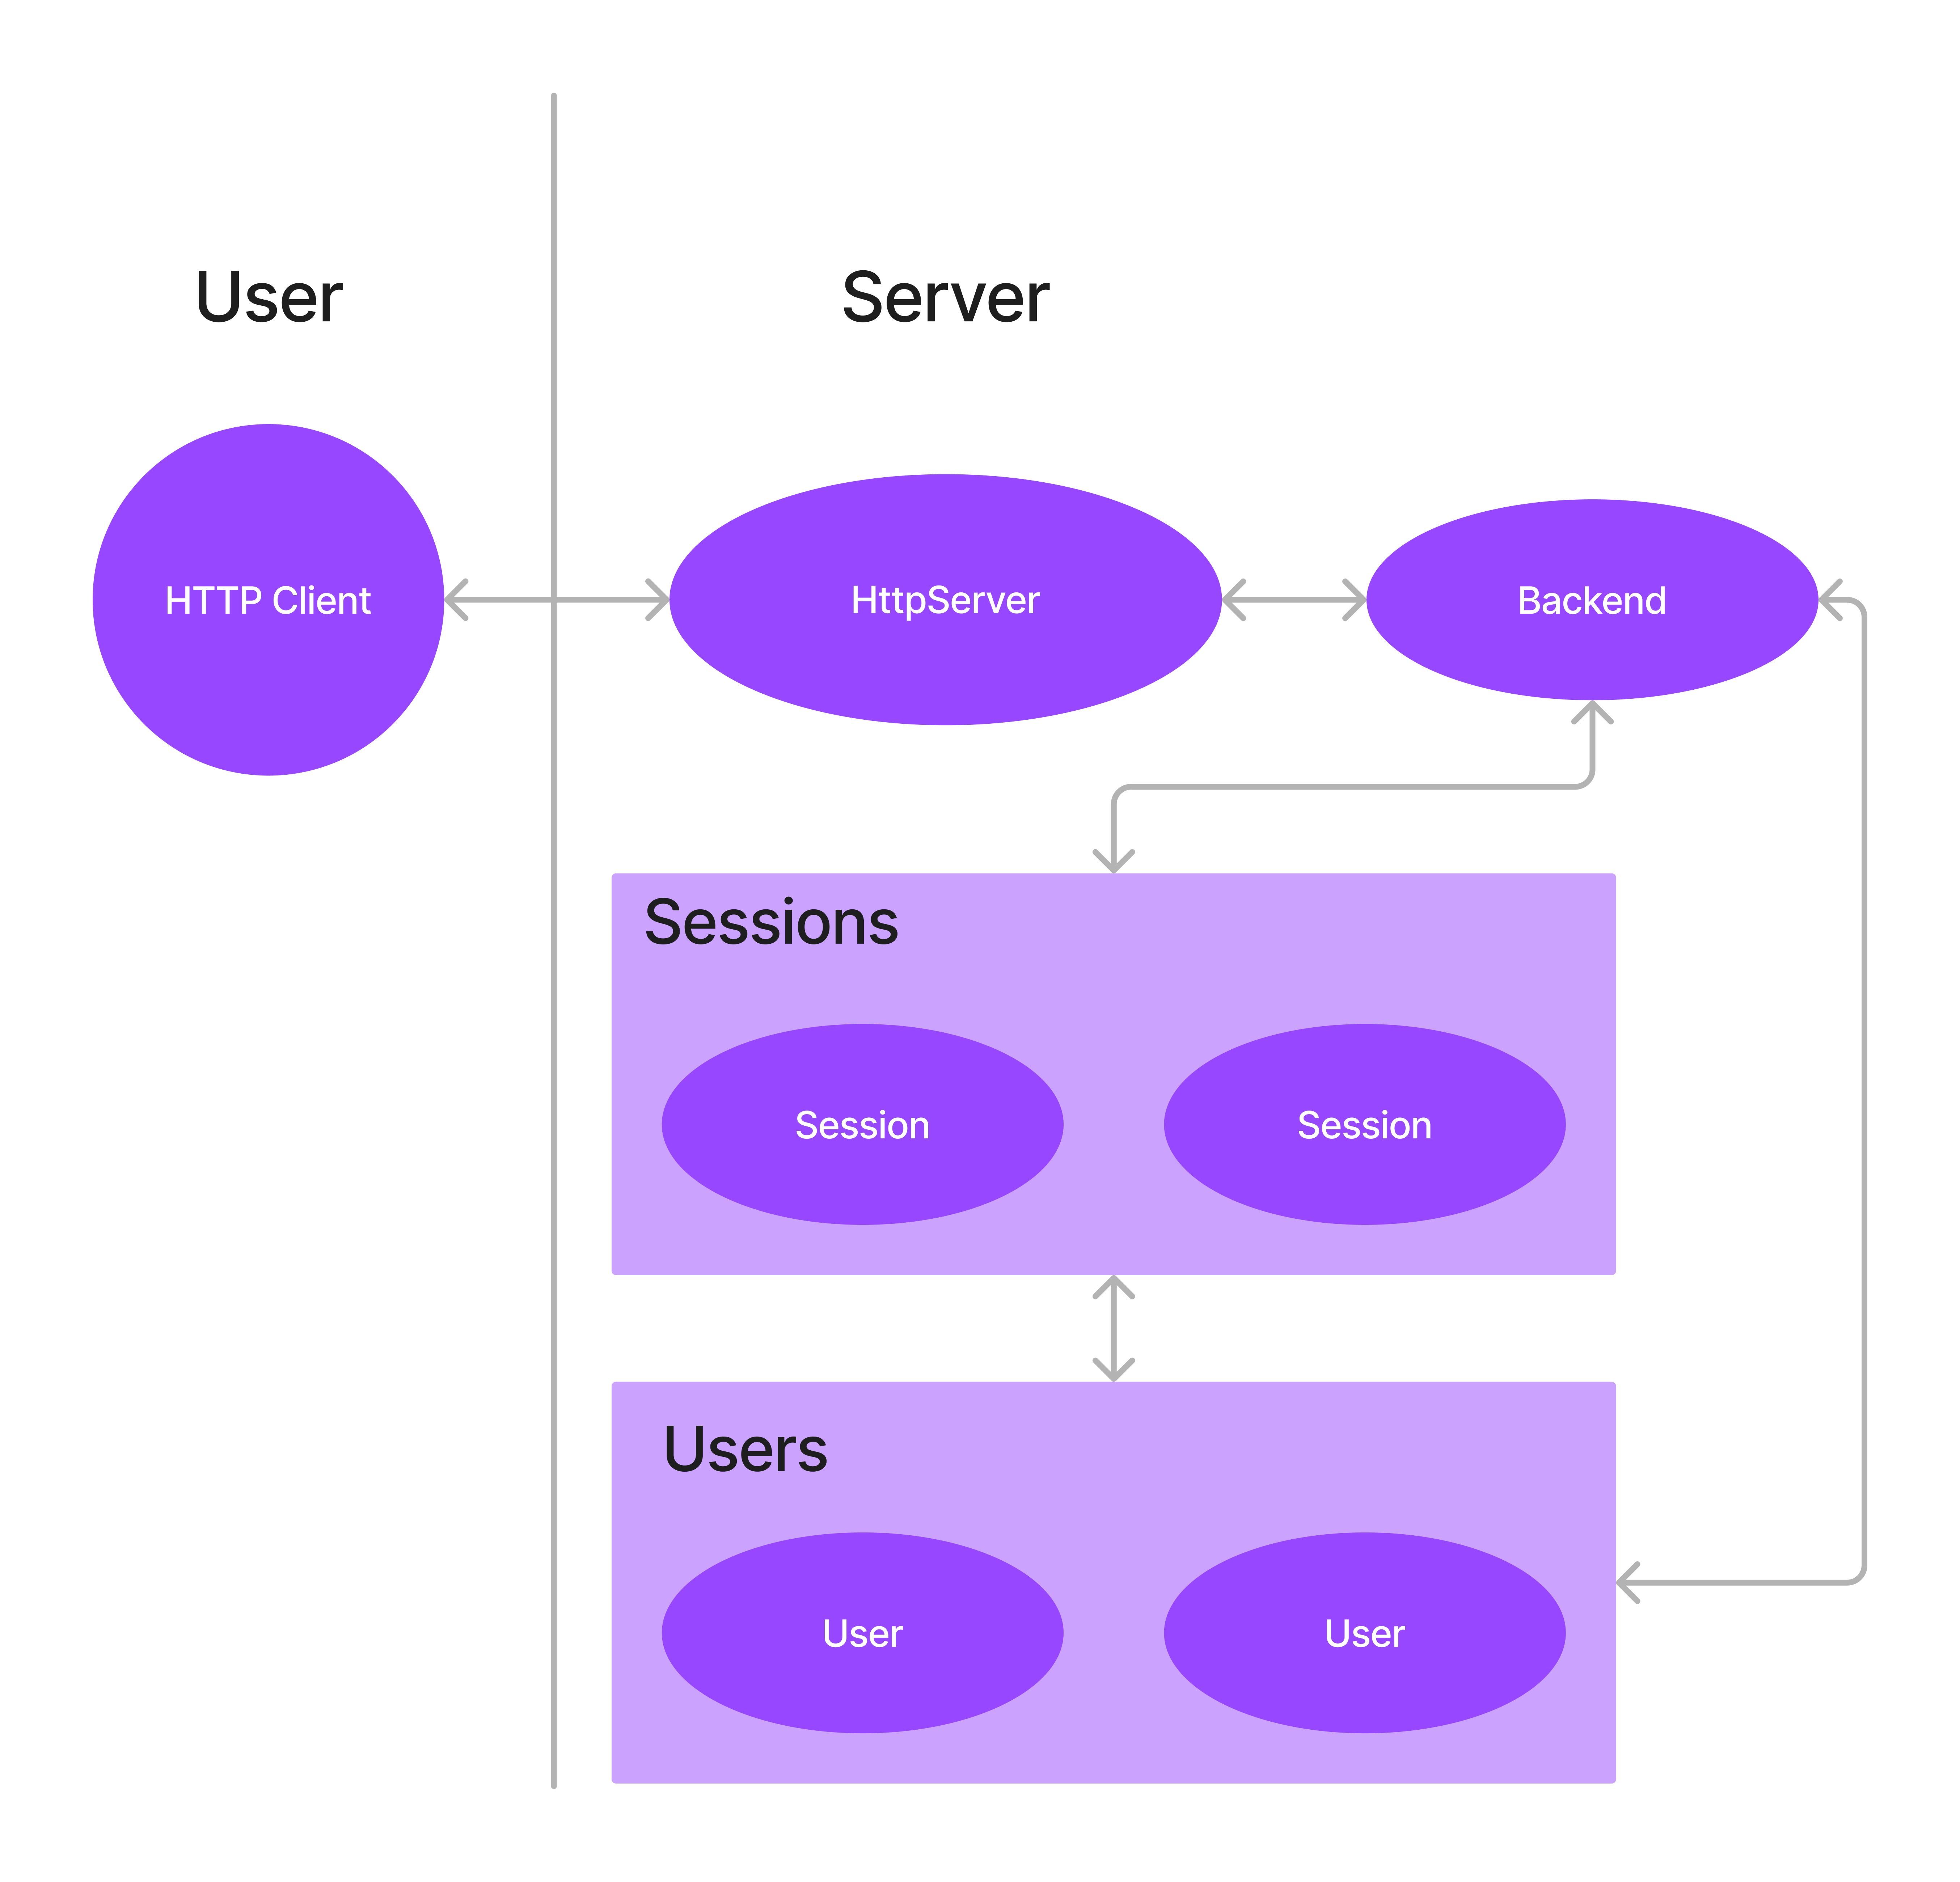
\includegraphics[width=\textwidth]{img/akka/HighLevel.png}
  \caption{Wysokopoziomowy schemat architektury serwera.}
  \label{fig:akka-highlevel}
\end{figure}

Serwer został zaimplementowany w języku Scala,
wykorzystując framework Akka \cite{Akka}.
Zaprojektowano dwupoziomową architekturę serwera
(Rys.~\ref{fig:akka-highlevel}).

Pierwszy poziom to serwer HTTP, który obsługuje
zapytania API oraz połączenia WebSocket.
Jest odpowiedzialny za tłumaczenie zapytań HTTP na
komunikaty wewnętrzne, które są przekazywane do
aktorów drugiego poziomu.
Za pomocą systemu autoryzacji JSON Web Token (JWT)
oraz serwisu Firebase Authentication,
serwer HTTP odczytuje identyfikatory $UserId$ oraz
$SessionId$ powiązane z~danym użytkownikiem.

%%% TODO powiekszenie schematow

\begin{figure}[!]
  \centering
  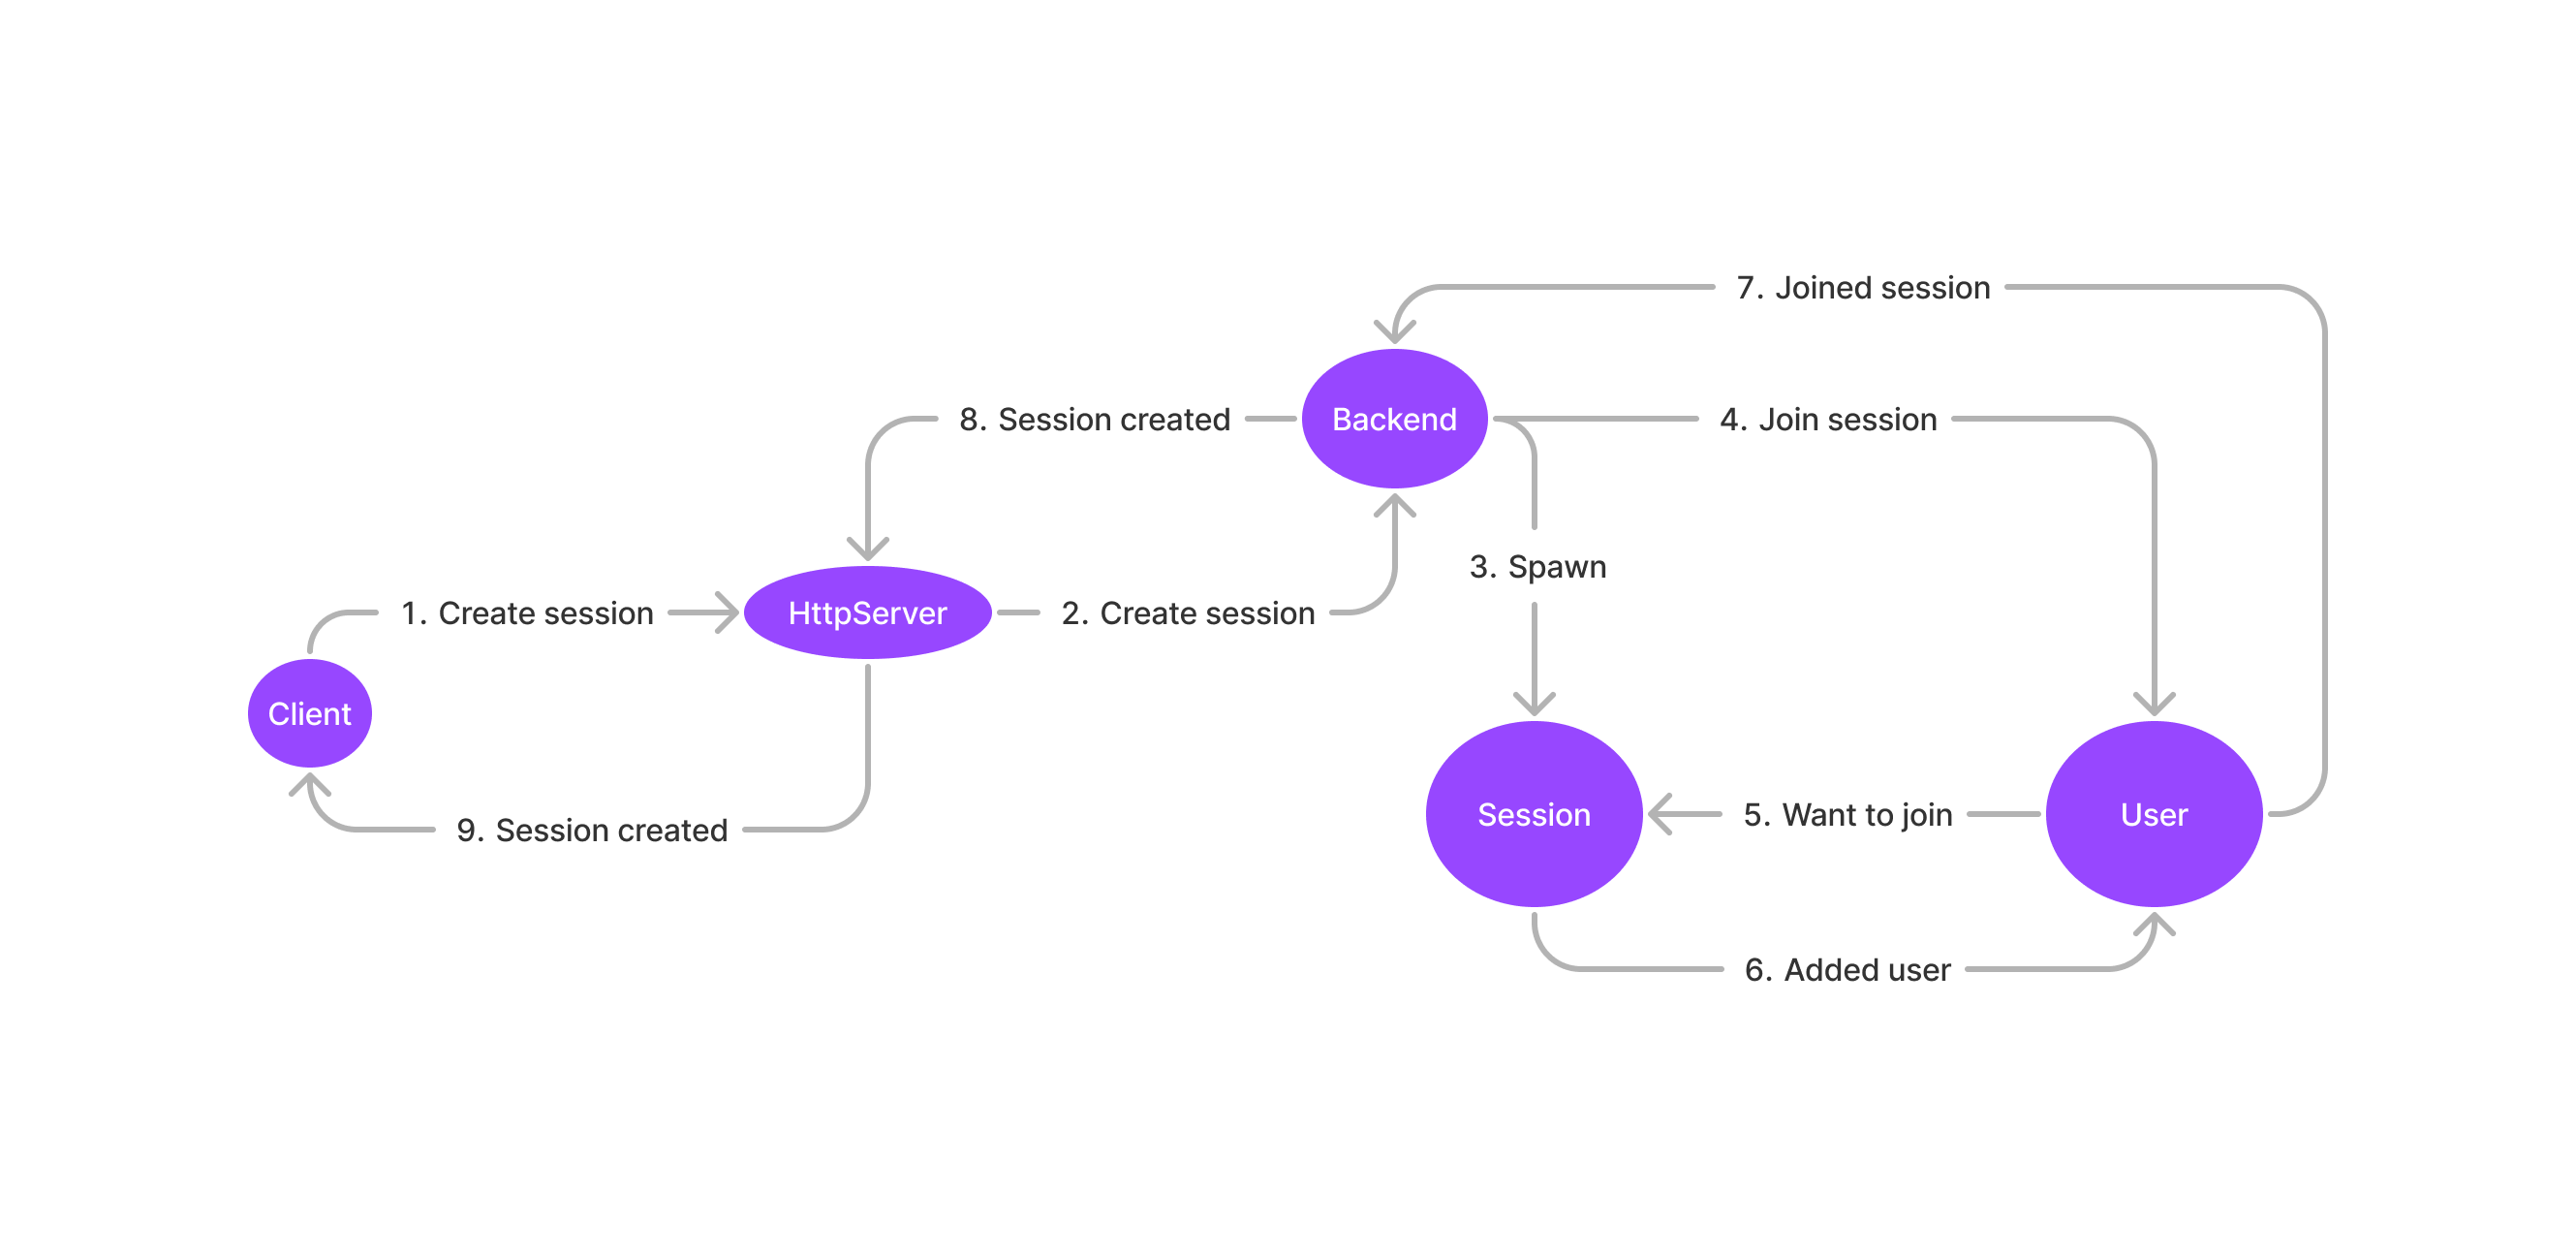
\includegraphics[width=\textwidth]{img/akka/CreateSession.png}
  \caption{Schemat tworzenia sesji.}
  \label{fig:akka-createsession}
\end{figure}

\begin{figure}[!]
  \centering
  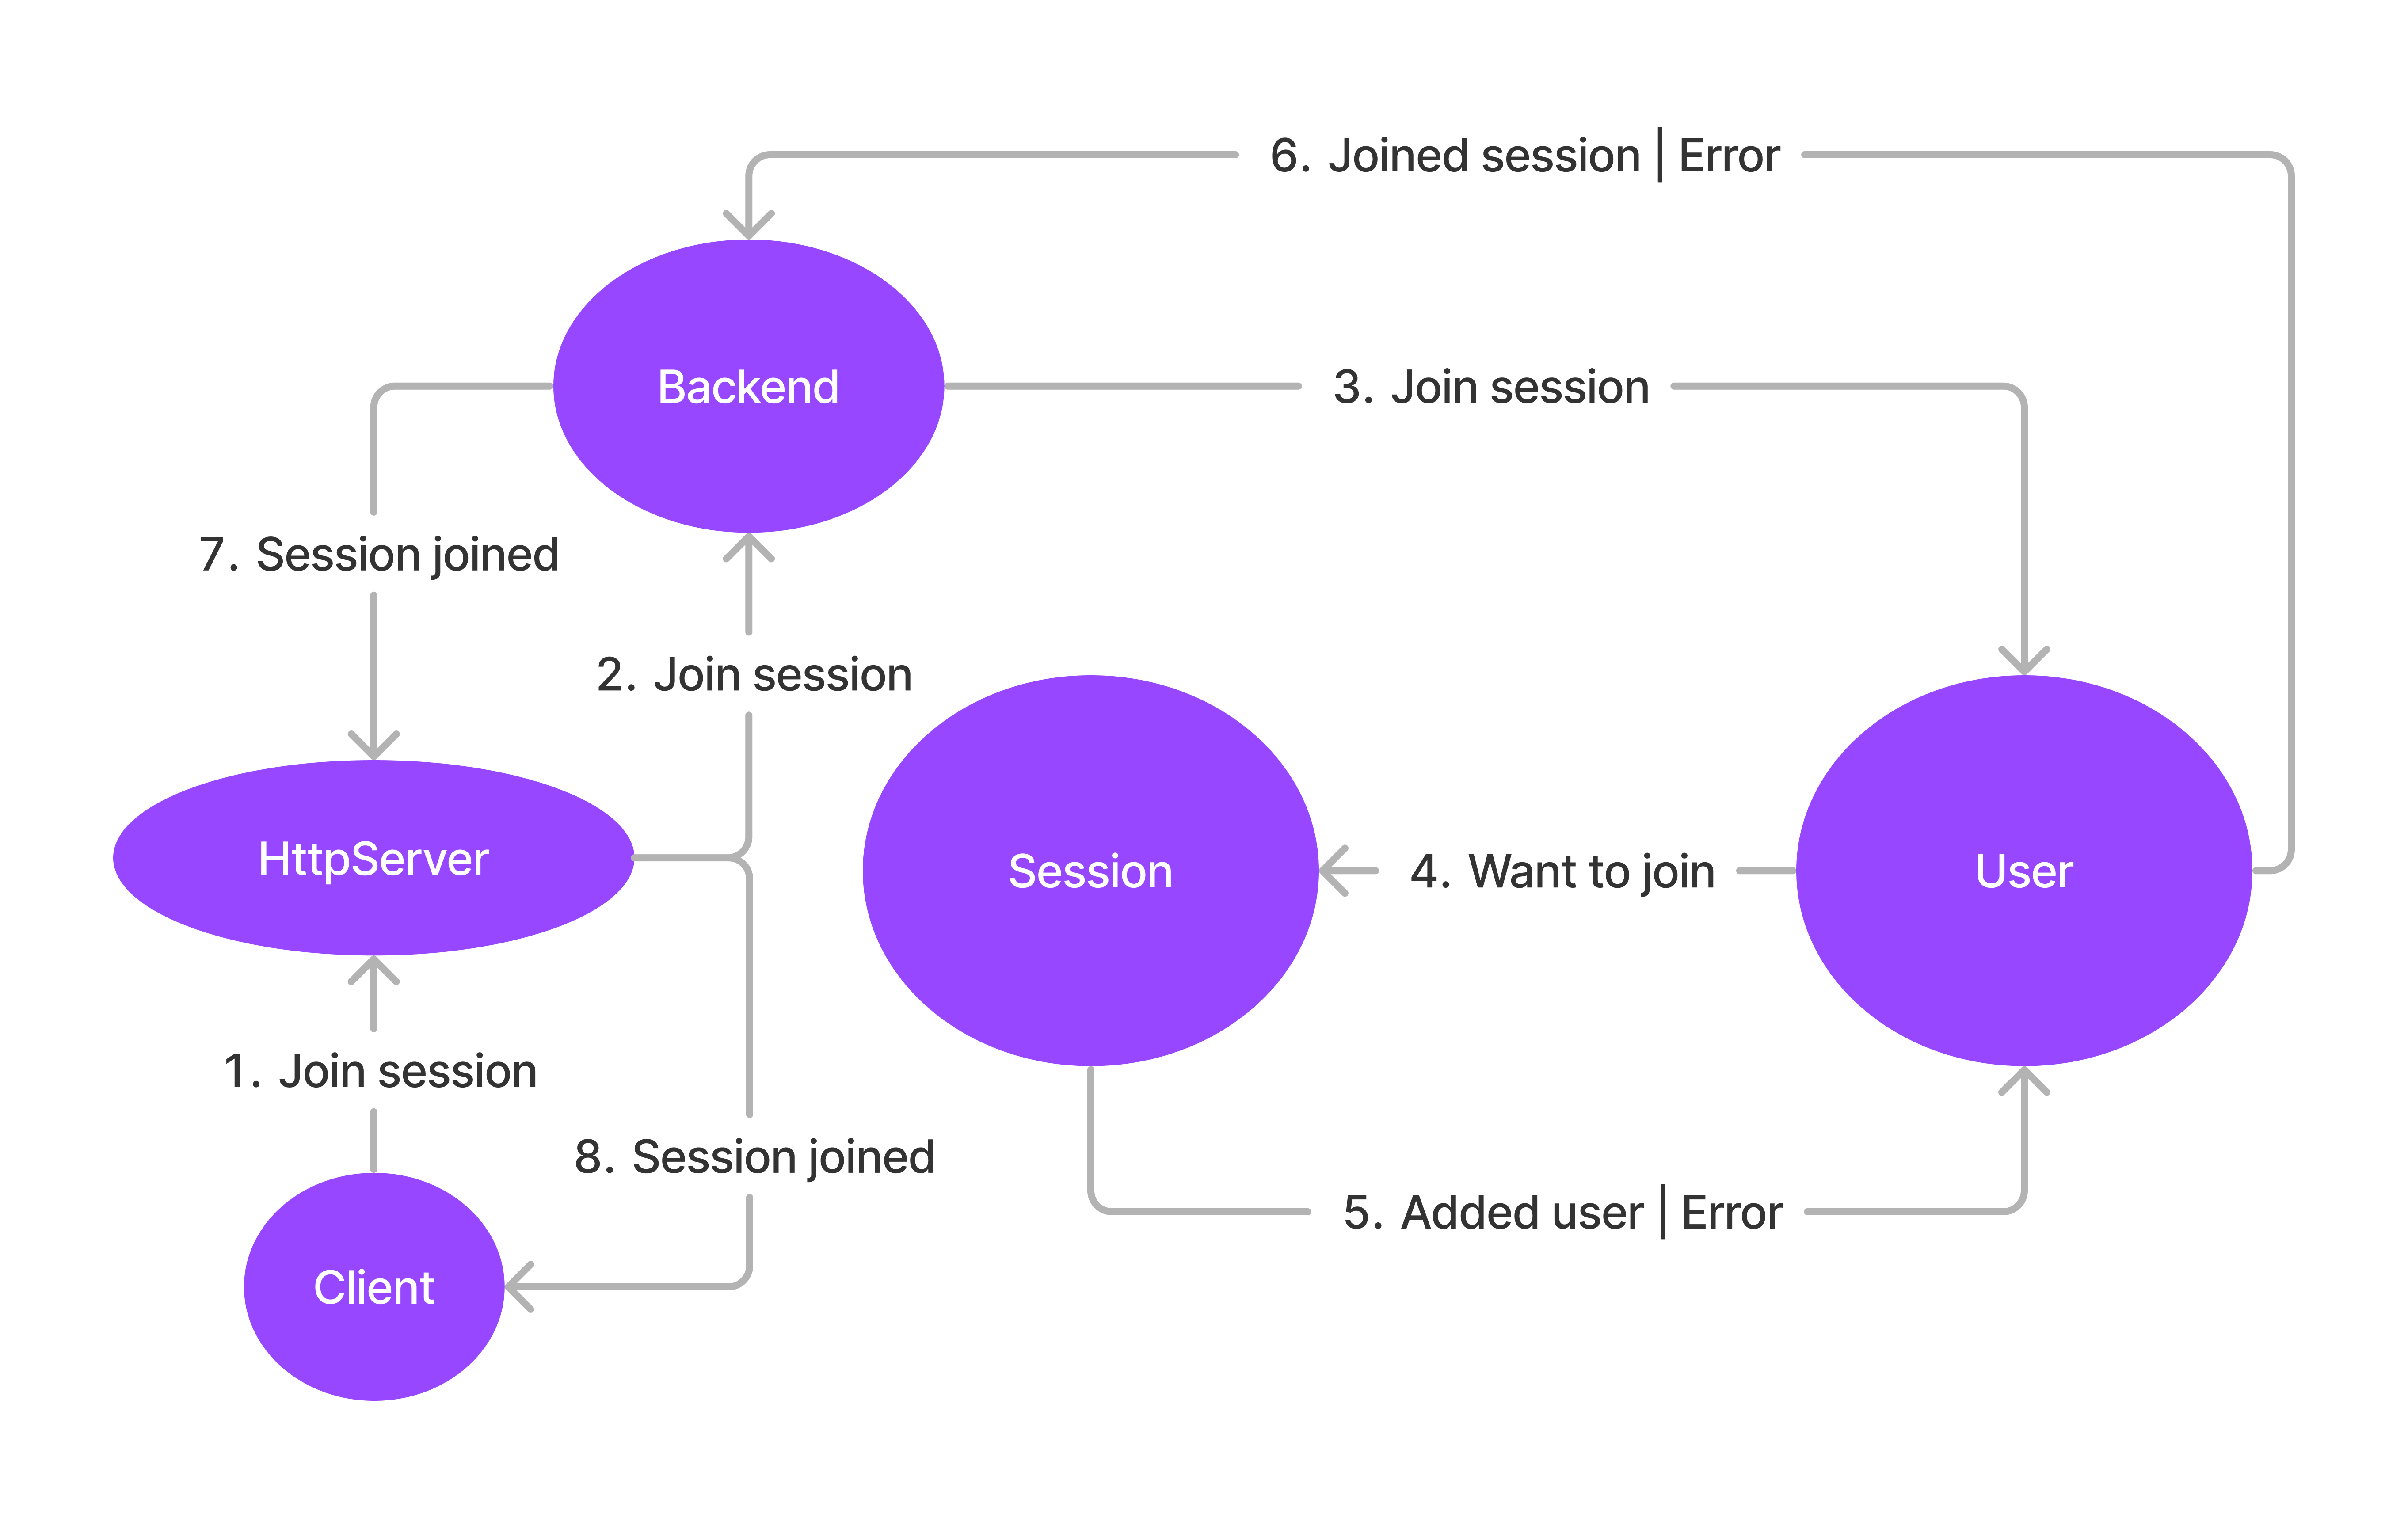
\includegraphics[width=\textwidth]{img/akka/JoinSession.png}
  \caption{Schemat dołączania do sesji.}
  \label{fig:akka-joinsession}
\end{figure}

\begin{figure}[!]
  \centering
  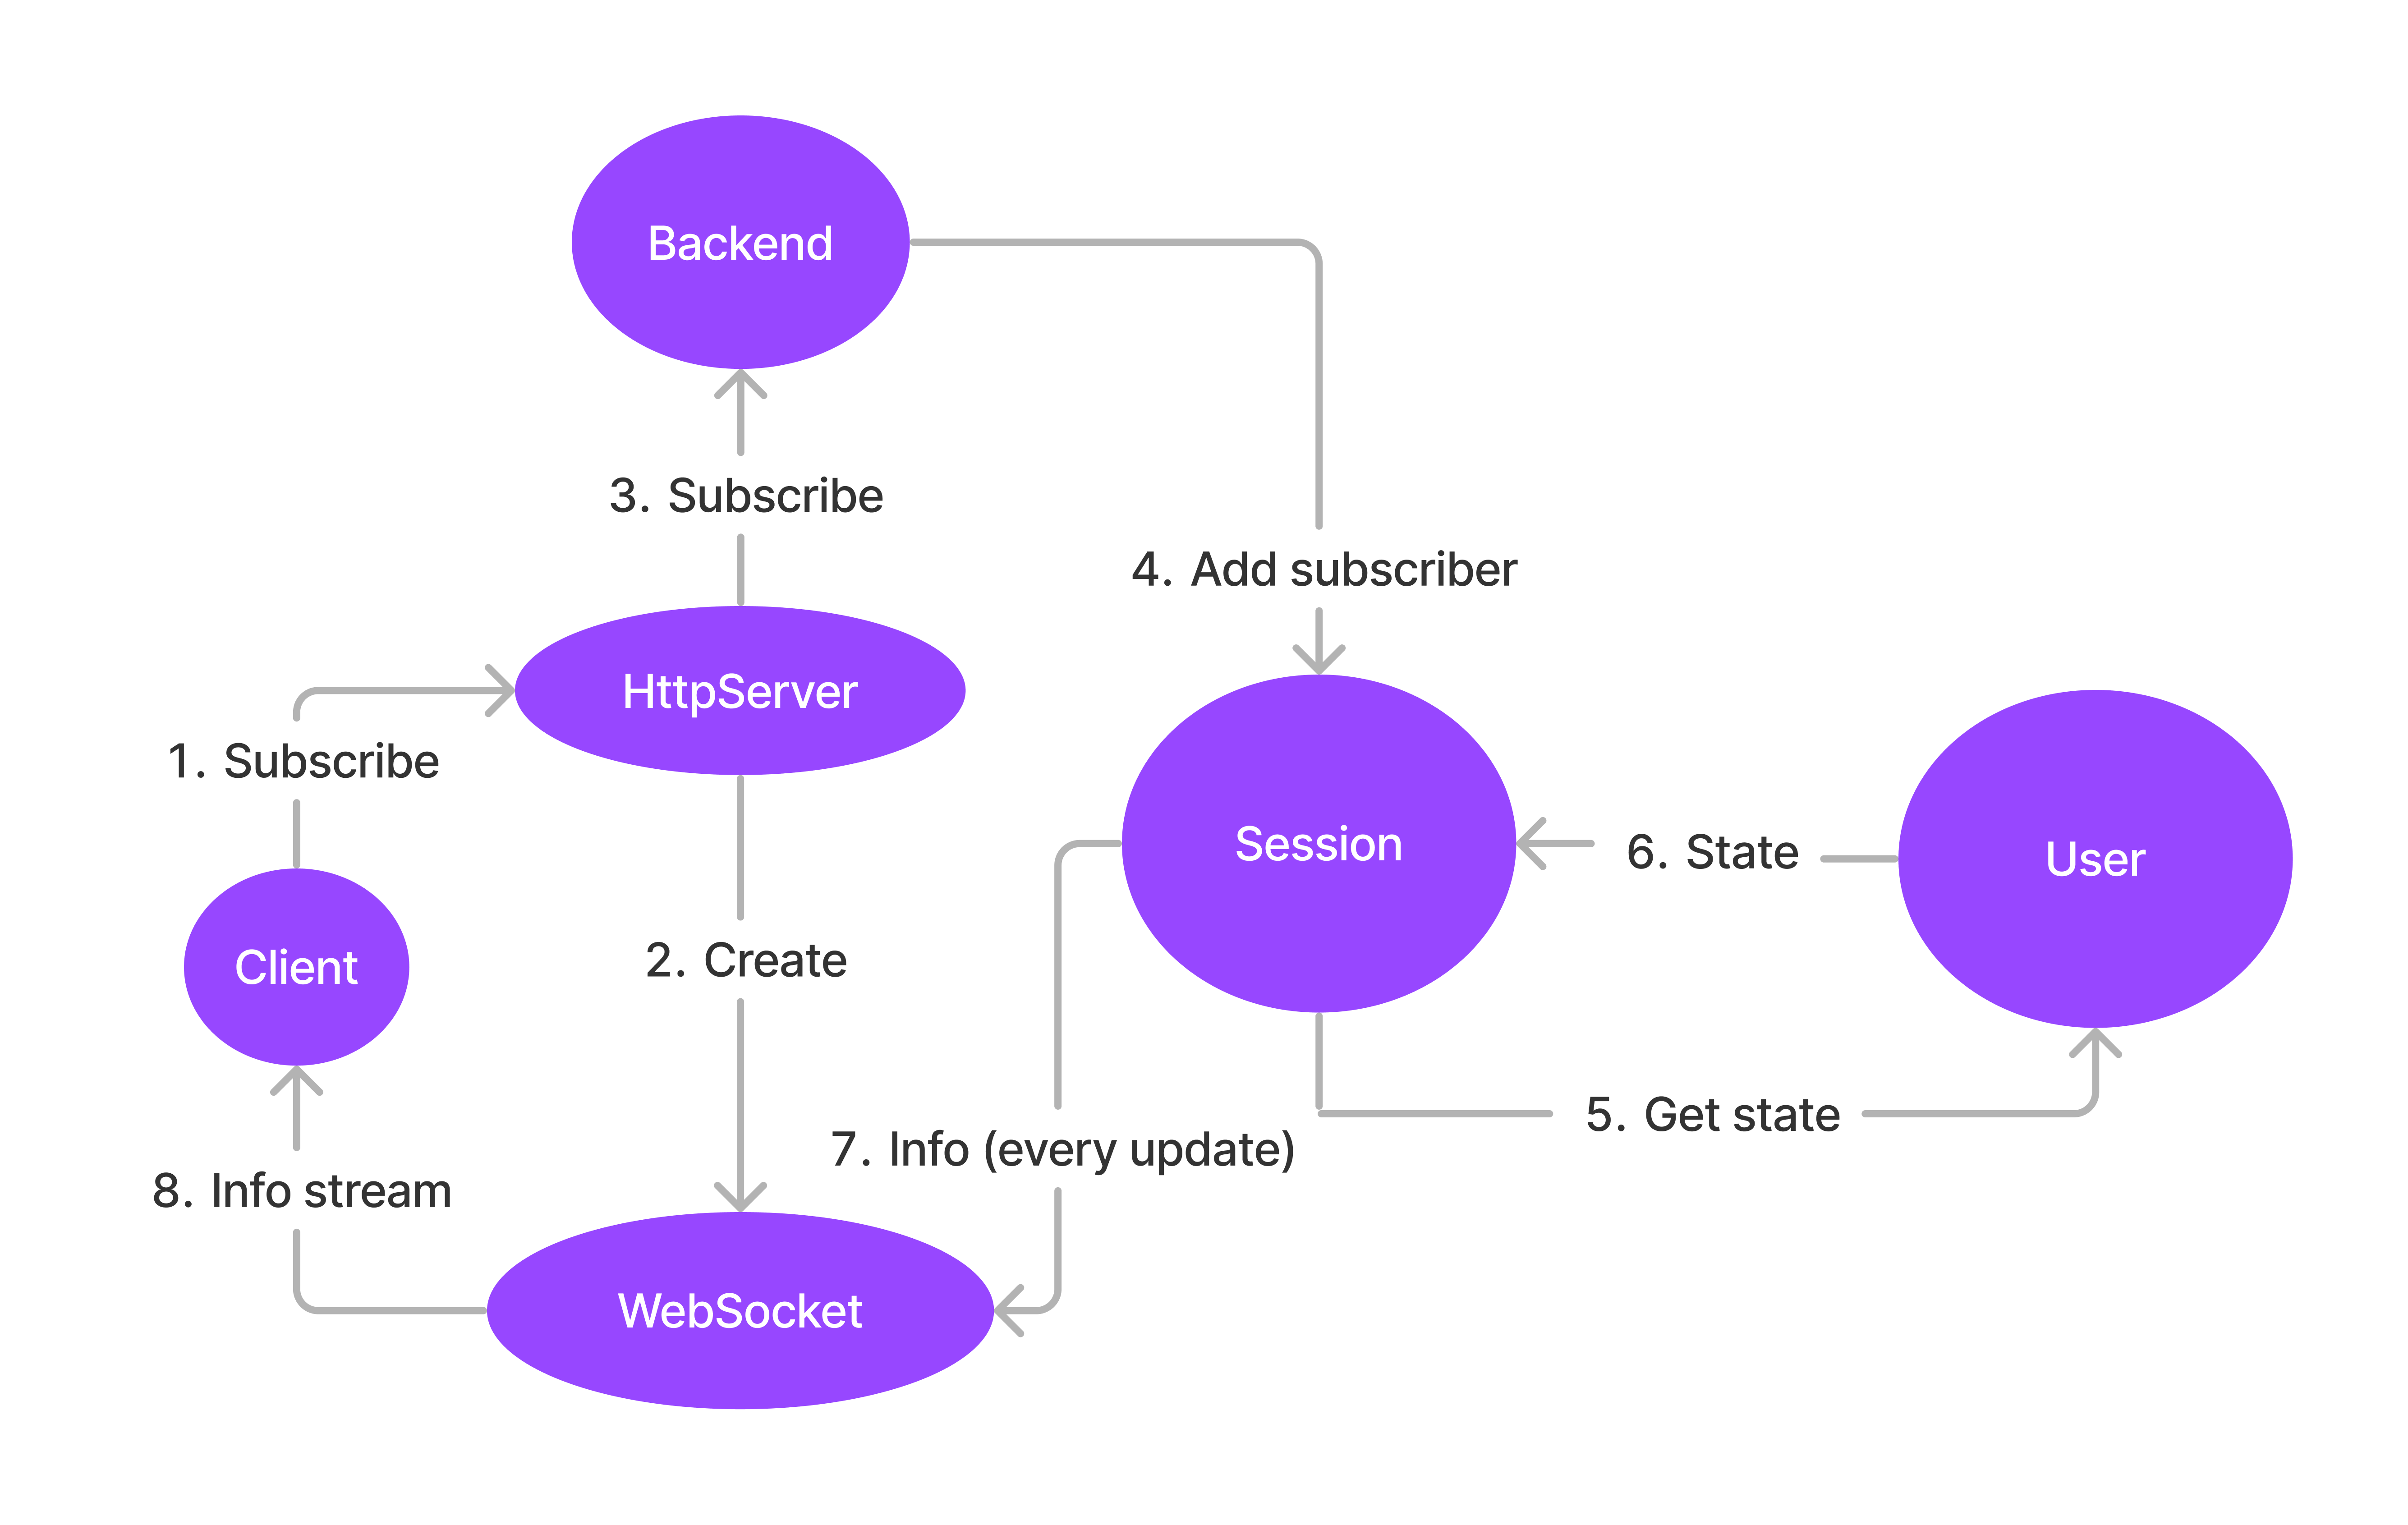
\includegraphics[width=\textwidth]{img/akka/SessionInfo.png}
  \caption{Schemat pobierania informacji o sesji.}
  \label{fig:akka-sessioninfo}
\end{figure}

Drugi poziom to system aktorów, który jest
odpowiedzialny za logikę biznesową.
Główny aktor \verb|Backend| zarządza mapowaniami
$SessionId \to Session$ oraz $UserId \to User$.
Każda sesja i~użytkownik reprezentowane są
przez własnego aktora.
Aktor \verb|Backend| wysyła komendy sterujące do
aktorów \verb|User|, którzy sami zarządzają swoim stanem.
Zaimplementowano obsługę błędów wynikających z~podania
niepoprawnych danych przez użytkownika.
Komunikaty wykorzystywane w~tym celu mają postać
\verb|Either[Error, Success]|.
Pozostałe błędy będące wynikiem wewnętrznych błędów
serwera są obsługiwane przez odrzucenie błędnego
komunikatu oraz przez mechanizm timeout.
W~takim przypadku klient uzyska odpowiedź
\verb|HTTP Timeout|, a~serwer pozostanie w~poprawnym stanie.
Cały protokół aktorów oraz ich maszyny stanowe zaprojektowane
zostały tak, aby uniemożliwić wystąpienie niespójności stanu serwera.
Schematy wybranych interakcji Klient-Serwer zostały przedstawione
na rysunkach \ref{fig:akka-createsession} -- \ref{fig:akka-sessioninfo}.

\FloatBarrier

\subsection{Komunikacja z serwerem}
Wstępne założenia dotyczące infrastruktury aplikacji
serwerowej opierały się na wykorzystaniu języka Python
wraz z~frameworkiem FastAPI.

Ze względu na problemy komunikacyjne aplikacji
z~serwerem, zdecydowano się na skonstruowanie struktury serwera
w~dynamicznym języku Scala, korzystając z~potencjału
frameworka Akka, specjalizującego się w~programowaniu
współbieżnym oraz rozproszonym, bazującym na
zaawansowanym modelu aktorów.

Pierwotny model komunikacji między klientem a~serwerem
był zbudowany w~oparciu o~metodę \textbf{short polling},
%%% TODO jakiś słownik co znaczy short polling???
zaimplementowaną przy pomocy FastAPI. Ten sposób
w~praktycznym zastosowaniu ujawnił pewne ograniczenia.
Regularne zapytania wysyłane przez klienta w~celu
sprawdzenia stanu danych na serwerze prowadziły do
znacznych opóźnień w~aktualizacji interfejsu
użytkownika. Taka sytuacja stwarzała trudności nawet
przy realizacji bardzo prostych funkcji, takich jak
zmiana pozycji użytkowników w~przestrzeni lobby.

Wobec wyzwań, narzuconych przez ograniczenia wyżej wspomnianej metody, nasz
zespół rozważał migrację ku strategii \textbf{long polling}. Metoda ta,
w~odróżnieniu od konwencjonalnych technik polegających na ciągłym
wysyłaniu zapytań przez klienta w~celu odświeżenia danych, proponuje
utrzymanie otwartego kanału HTTP do czasu, aż serwer będzie miał
najnowsze informacje do przekazania. Mimo iż koncepcja ta wydawała się
obiecująca, powstały obawy związane z~koniecznością ciągłego monitorowania
potencjalnej utraty połączenia. Skłoniło nas do ostatecznej rezygnacji
z~wdrożenia tego pomysłu.

Implementacja frameworka Akka \cite{Akka} pozwoliła na ustanowienie stabilnego,
reaktywnego połączenia między klientem a~serwerem. Programowanie
reaktywne, koncentrujące się na płynnym przepływie danych i~ich propagacji,
umożliwiło aplikacji klienta natychmiastowo reagować na wszelkie zmiany. Jest
to szczególnie istotne w~kontekście naszej aplikacji, która charakteryzuje
się intensywną interakcją użytkownika, zwłaszcza podczas naszej kluczowej
funkcjonalności -- rozgrywki w~brydża. Zastosowanie tego podejścia
znacząco usprawniło koordynację sekwencji animacji ruchów poszczególnych
graczy.

%%% mozna opisac to pozniej
% \subsection{Testy}
% Framework Akka dostarcza także kompleksowe narzędzia do efektywnego
% testowania aktorów, w~tym symulowane środowisko czasu wykonania, które
% pozwala na dogłębne sprawdzenie zachowań asynchronicznych w~warunkach
% synchronicznych. Dzięki tym możliwościom możemy rozwijać architekturę
% serwera, mając pełne przekonanie co do jej stabilności i~niezawodności
% działania.

\section{Aplikacja webowa}
Aplikacja webowa została stworzona przy użyciu platformy Next.js
\cite{NextJS} oraz języka programowania Typescript \cite{Typescript},
będącego rozszerzeniem języka JavaScript o~statyczne typowanie.
Jednakże ze względu na problemy wydajnościowe rozgrywki
i~słabą responsywność interfejsu związaną z~połączeniem serwerowym
zdecydowano się na zmianę technologii odpowiedzialnych za te zadania.

Implementacja rozgrywki w~brydża została logicznie
odseparowana od reszty aplikacji, choć w~pełni integruje się z~samą
platformą i~korzysta z~wcześniej wspomnianych języków programowania.
Szczegółowy opis części znajduje się w~podrozdziale \nameref{subsec:silnik_gry}.

\subsection{Mechanizmy stanu i cyklu życia komponentów}
Biblioteka React oferuje narzędzie w~postaci \textbf{hooków},
które umożliwiają efektywne zarządzanie stanem i~cyklem życia komponentów.
Są to funkcje, które udostępniają stany obiektów, oferując do nich wgląd, automatyczną aktualizację
lub zmianę wartości stanów.

W~naszym projekcie, do obsługi zapytań klienta do serwera, zdecydowaliśmy się
skorzystać z~biblioteki SWR \cite{SWR}.
Jest to rozwiązanie, korzystające z~hooków, do
pobierania danych rozwiązujące wiele problemów implementacynych takich jak
cache'owanie i~deduplikacje (usuwanie redundantnych kopii) danych, ponawianie żądań
czy weryfikacja połączenia po odzyskaniu dostępu do sieci.

Aby jeszcze bardziej zoptymalizować proces, stworzyliśmy
również zestaw własnych, dedykowanych hooków. Takie podejście pozwoliło na
znaczną standaryzację logiki odpowiedzialnej za aktualizacje stanów przy pomocy
zapytań HTTP z~użyciem SWR. Przyczyniło się do zmniejszenia ilości
globalnych zmian kodu, gdyż zmiana implementacji nie zmieniła samego interfejsu
hooka. Funkcjonalność pozostała niezmienna i~oferowane stany miały taką samą strukturę.

Jak zostało wspomniane we wcześniejszym podrozdziale, dotyczącym serwera aplikacji,
zrezygnowano ze wspomnianego rozwiązania biblioteki SWR na rzecz reaktywnego
połączenia z~serwerem. Wymusiło to zmianę implementacji wysyłania i~odbierania
zapytań do serwera. Logika
wykorzystania hooków pozostała taka sama, przez co komponenty interfejsu
zawierające wspomniane hooki nie musiały być aktualizowane po tej zmianie. \\

Poniżej przedstawione zostały hooki odpowiedzialne za aktualizacje
danych z~serwera, wykorzystując Fetch API \cite{FetchAPI} do wysyłania pojedynczych
zapytań i~WebSockety \cite{WebSockets} do ustanawiania połączenia z~serwerem
i~ciągłą aktualizację oferowanego stanu przez serwer.

\begin{lstlisting}[language=JavaScript, caption=Hooki z Fetch API, label={lst:fetch-hooks}, captionpos=b]
export function useFetch<T, U>(fetcher: (request: T) => Promise<U>): FetchState<T, U> {
  const [data, setData] = useState<U | undefined>(undefined);
  const [loading, setLoading] = useState<boolean>(false);

  const trigger = useCallback((request: T) => {
    if (loading) return Promise.reject();
    setData(undefined);
    setLoading(true);
    return fetcher(request)
      .then(data => {
        setData(data);
        return data;
      })
      .finally(() => {
        setLoading(false);
      });
  }, [fetcher, loading]);

  return { trigger, data, loading };
}

async function createLobbyFetcher(unused: void): Promise<CreateLobbyResponse> {
  const token = await getIdToken();
  const res = await fetch($`$$\dollar${API_URL_SESSION_LOBBY}/create$`$, {
    method: "POST",
    headers: {
      "Content-Type": "application/json",
      "Authorization": $`$Bearer $\dollar${token}$`$
    },
  });
  if (!res.ok) return Promise.reject(res.statusText);
  return res.json();
}

export function useCreateLobby() {
  return useFetch(createLobbyFetcher);
}
\end{lstlisting}

\vspace*{0.5cm}

\begin{lstlisting}[language=JavaScript, caption=Hooki z WebSocketem, label={lst:websocket-hooks}, captionpos=b]
export function useSocket<T>(url: string | undefined): SocketState<T> {
  url = url?.replace(/^http/, "ws");

  const [data, setData] = useState<T | undefined>(undefined);
  const loading = data === undefined;

  const getAuthUrl = useCallback(() => {
    return getIdToken().then(token => {
      return $`$$\dollar${url}?access_token=$\dollar${token}$`$;
    });
  }, [url]);

  useWebSocket(url ? getAuthUrl : null, {
    shouldReconnect: () => true,
    onMessage: (event) => {
      setData(JSON.parse(event.data));
    },
    reconnectInterval: 500,
  });

  return { data, loading };
}  

export interface GetInfoResponse {
  sessionId: string
  hostId: string
  users: Player[]
  started: boolean
  gameState: GameState | null
}

export function useSessionInfo(): SocketState<GetInfoResponse> {
  return useSocket<GetInfoResponse>($`$$\dollar${API_URL_SESSION}/info$`$);
}

\end{lstlisting}

\subsection{Stylizacja interfejsu}
W~celu nadania stylów komponentom naszej aplikacji internetowej posłużono się
frameworkiem Tailwind CSS. W~połączeniu z~biblioteką Daisy UI
\cite{DaisyUI}, która
w~pełni wspiera ten framework, możliwe było zastosowanie gotowych klas
stylistycznych. Oferują one nie tylko samą edycję pojedynczych elementów, ale też
utworzenie zaprojektowanych, w~pełni animowanych obiektów.

Ze względu na intuicyjne nazewnictwo klas stylizujących możliwe było szybkie
projektowanie interfejsu użytkownika i~wyeliminowało
potrzebę bezpośredniego zarządzania plikami CSS. Jest to szczególnie
przydatne, jeżeli wykorzystywany jest React, ze względu na jego naturalny podział
elementów na osobne komponenty. Wykorzystanie tego podejścia znacznie przyspieszyło
proces rozwoju części wizualnej aplikacji.


\section{Silnik gry}
\label{subsec:silnik_gry}

Silnik wizualny rozgrywki do gry w~brydża jest kluczowym elementem aplikacji.
Podczas tworzenia go skupiono się, aby zaoferować
wysoką wydajność i~pełną integrację z~aplikacją webową.


\subsection{Framework Three.js}

Podczas tworzenia środowiska gry, powstał problem z~zarządzaniem
elementami kart i~ich przemieszczaniem na ekranie użytkownika. Animacje,
takie jak ruch kart, z~wykorzystaniem wyłącznie komponentów React
okazały się nadmiernie pracochłonne i~nieefektywne. Użytkownik
mobilny miał problemy z~ładowaniem kart
i~ich płynnym animowaniem w~przeglądarce. Jest to spowodowane inną architekturą procesorów
mobilnych w~porównaniu do rozwiązań desktopowych. Nie są one przystosowane
do wykonania najmocniejszych obliczeń, ale oferują niskie zużycie energii.
Również na wydajność wpłynęło wykorzystanie grafik wektorowych SVG,
które podczas animacji bardzo obciążały przeglądarkę i~zmniejszały
ich płynność. \\

Wymusiło to rezygnację z~rozwiązania wykorzystującego jedynie elementy HTML.
Dokonano zmiany na framework umożliwiający renderowanie
środowiska i~elementów
\mbox{3D -- Three.js~\cite{ThreeJS}~(Rys.~\ref{fig:engine_orbit})}.

\begin{figure}[hbt!]
  \centering
  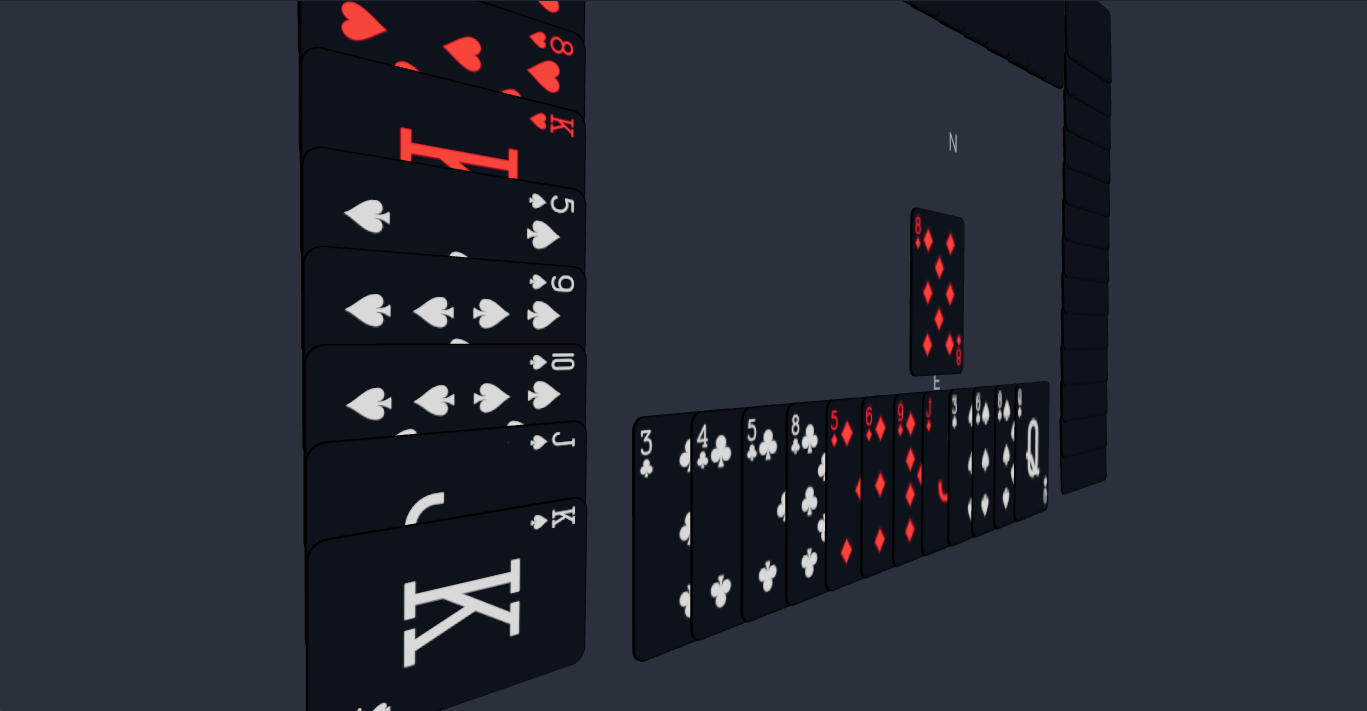
\includegraphics[width=0.9\textwidth]{img/bridge-engine/orbit.png}
  \caption{Widok boczny trójwymiarowej przestrzeni silnika gry.}
  \label{fig:engine_orbit}
\end{figure}

Posiada on wszystkie potrzebne funkcje, które pozwalają na zaawansowane
zarządzanie aspektami wizualnymi. Udostępnia on:
\textit{canvas} -- którego zadaniem jest zdefiniowanie
obszaru, na którym znajdują się wyświetlane elementy;
\textit{przestrzeń 3D} - w której możemy umieszczać
karty i~przemieszczać niezależnie od struktury komponentów;
\textit{kamerę} -- pozwalającą na wykorzystanie perspektywy
w~środowisku 3D, przez co gracze mogą mieć wizualne
odczucie realnej rozgrywki gry w~brydża.

Dodatkowo framework ten został wybrany ze względu na swoją wydajność.
Do renderowania elementów wykorzystuję on potencjał WebGL \cite{WebGL}.
Jest to API utworzone
w~języku JavaScript, które jest standardem webowym wykorzystywanym
w~przeglądarkach. Umożliwia ono wykorzystanie akceleracji sprzętowej kart
graficznych, które są przystosowane do przetwarzania fizyki, zdjęć
i~efektów wizualnych. Kluczowe jest, że stosując wspomnianą akcelerację,
wykorzystujemy większe możliwości sprzętowe urządzeń mobilnych, jak
i~desktopowych, które nie były w~pełni wykorzystywane z~użyciem
jedynie elementów HTML.
Zastosowanie tego rozwiązania
znacznie zwiększyło efektywność i~płynność silnika gry na tych urządzeniach.
Przykładowo badając skok wydajności, porównując pierwotny silnik z~obecnym,
na urządzeniu mobilnym, różnica jest na poziomie od około 15 aż do
ponad 140 wyświetlanych
klatek na sekundę\footnote{
  Porównanie zostało wykonane na urządzeniu
  Samsung Galaxy S10+ z procesorem Samsung Exynos 9820.
}.

\FloatBarrier

\subsection{Integracja silnika z Reactem}
Three.js oprócz wspomnianych zalet jest też wspierany w~postaci komponentów React.
Rozwiązania, które są wykorzystane w~aplikacji to React Three Fiber
\cite{ReactThreeFiber} i~React drei \cite{ReactDrei}. Oba oferują
wspomniane komponenty, jak i~dodatkowe moduły
wspomagające prace Three.js w~środowisku React. Uniknięto w~ten sposób korzystania
z~JavaScript'a, a~wykorzystano oferowane hooki i~komponenty.



\section{Wirtualny asystent}

Główne funkcje wirtualnego asystenta wykorzystują informację o najlepszych ruchach
dostępnych dla gracza w danym momencie rozgrywki.
W ten sposób może on pełnić funkcję wirtualnego gracza lub
udzielać wskazówek graczom w trakcie rozgrywki.
Analiza najlepszych ruchów wykorzystuje dedykowane algorytmy AI
do fazy licytacji i~fazy gry.

\subsection{Faza licytacji}

Licytacja w~brydżu jest otwartym problemem w~dziedzinie AI.
Pozostaje ona wyzwaniem dla naukowców.
Zdecydowano się na implementację algorytmu AlphaZero \cite{AlphaZeroPaper},
po przystosowaniu do gry w~brydża.

\subsubsection{AlphaZero}

AlphaZero jest algorytmem uczenia maszynowego, który rozwija
algorytm Monte Carlo Tree Search (MCTS) o~sieć neuronową do ewaluacji
stanów gry.
Analogicznie do MCTS, AlphaZero eksploruje drzewo stanów gry,
symulując możliwe ruchy wszystkich graczy.
MCTS ocenia jakość stanu metodą Random Rollout, czyli
losowym symulowaniem ruchów do końca gry.
AlphaZero ocenia stan gry za pomocą sieci neuronowej $v$.
Druga sieć neuronowa $\pi$ przewiduje rozkład
prawdopodobieństwa wyboru każdego ruchu.
W~implementacji obie sieci neuronowe są połączone w~jedną
sieć o dwóch wyjściach.
Dodatkowo zastosowano modyfikację
Gumbel AlphaZero \cite{GumbelAZ},
która gwarantuje poprawę funkcji polityki $\pi$, pod warunkiem
dobrej oceny stanu $v$.


\subsubsection{Przystosowanie do gry w~brydża}

Formalnie, brydż to gra:
\begin{itemize}
  \item czteroosobowa,
  \item niedeterministyczna,
  \item o sumie zerowej,
  \item z~niepełną informacją.
\end{itemize}

AlphaZero został zaprojektowany do gier:
\begin{itemize}
  \item dwuosobowych,
  \item deterministycznych,
  \item o sumie zerowej,
  \item z~pełną informacją.
\end{itemize}

W brydżu występuje szczególny przypadek niedeterminizmu,
czyli niedeterminizm konfiguracji początkowej.
Skutki wykonania każdego ruchu są deterministyczne,
natomiast początkowe rozdanie kart podlega losowości.
Z tego powodu możemy traktować fazę gry po rozdaniu jako
grę deterministyczną.

Algorytmy MCTS i~AlphaZero wymagają pełnej informacji o~stanie gry.
W~brydżu gracz nie zna kart przeciwników i~partnera.
Z~tego powodu nie jest możliwe symulowanie ruchów przeciwników.
Dokonano pewnej obserwacji, która pozwala użyć AlphaZero do gier
z~niepełną informacją.
AlphaZero wykorzystuje sieć neuronową $\pi$ do predykcji
prawdopodobieństwa wyboru każdego ruchu.
Sieć $\pi$ uczona jest poprzez minimalizację funkcji kosztu,
która zdefiniowana jest jako entropia krzyżowa pomiędzy
przewidzianym rozkładem a~wynikiem algorytmu MCTS.
Sam MCTS również wykorzystuje $\pi$ jako rozkład
\textit{a~priori} w każdym węźle.
Finalny wynik MCTS po określonej liczbie iteracji
to rozkład prawdopodobieństwa wyboru każdego ruchu,
który maksymalizuje wartość oczekiwaną nagrody.
Dla stanów nieterminalnych nagroda jest przewidywana
przez sieć $v$.
Przy liczbie iteracji MCTS dążącej do nieskończoności,
algorytm zbiega się do rozwiązania MiniMax, czyli optymalnego.
Można zatem wnioskować, że sieć $\pi$ również zbiega się
do rozwiązania MiniMax, ponieważ \textit{internalizuje}
wyszukiwanie MCTS. W~literaturze MCTS opisywany jest jako
\textit{policy improvement operator} \cite{MuZeroPaper,EfficientZeroPaper},
czyli metoda poprawy funkcji $\pi$.
W~procesie uczenia sieć $\pi$ uczy się przewidywać wynik MCTS,
dlatego dla nieskończonej liczby iteracji MCTS,
sieć $\pi$ zbiega się do rozwiązania MiniMax.

Skoro udowodniono, że sieć $\pi$ uczy się przewidywać
optymalny ruch (pod kątem maksymalizacji oczekiwanej nagrody),
można wykorzystać samą sieć, bez MCTS, do wyboru ruchu.
W~praktyce MCTS zwraca lepszy wynik, ale wymaga
symulacji ruchów przeciwników.
W~naszym przypadku nie jest to możliwe, dlatego
zdecydowano się na wykorzystanie samej sieci $\pi$,
która w~czasie $O(1)$ wybiera ruch na podstawie obserwacji stanu gry.
Sieć była uczona za pomocą algorytmu MCTS (\textit{policy improvement operator}),
który znał pełny stan gry.
Sieć $\pi$ nie zna pełnego stanu gry, ale zna obserwację stanu gry
z~punktu widzenia jednego z~graczy.
Jest zatem w~stanie przewidzieć optymalny ruch,
mając dostęp jedynie do kart jednego gracza.

Analogicznie do \cite{rong19,gong20,tian20,lockhart20}, zastosowano
algorytm Double Dummy Solver (DDS) \cite{DDS} do generowania
nagród dla stanów terminalnych licytacji.
AlphaZero wymaga gier dwuosobowych.
W~brydżu uczestniczy czterech graczy w~dwóch drużynach.
Można zatem potraktować drużynę jako \textit{abstrakcyjnego gracza}.
Finalna nagroda zdefiniowana jest następująco:
\begin{itemize}
  \item 1 -- wygrana drużyny,
  \item 0 -- remis,
  \item -1 -- przegrana drużyny.
\end{itemize}
Każda drużyna podejmuje decyzje maksymalizujące swoją nagrodę.
W~przypadku kolejności \textit{fizycznych graczy}
N -- E -- S -- W, kolejność graczy abstrakcyjnych to
NS -- EW -- NS -- EW.
Można to interpretować jako grę dwuosobową,
gdzie gracze ,,przesiadają się'', zapominając o~swoich kartach.
Decyzje mogą być podejmowane tylko na podstawie kart, które
są widoczne dla gracza w~danej turze.
Taka modyfikacja gry pozwala na zastosowanie AlphaZero.

\subsubsection{Implementacja}

Algorytm AlphaZero został zaimplementowany w~języku Python,
wykorzystując biblioteki:
\begin{itemize}
  \item JAX \cite{JAX} -- backend do obliczeń numerycznych,
  \item Haiku \cite{Haiku} -- biblioteka do tworzenia sieci neuronowych,
  \item PGX \cite{PGX} -- implementacja gry w~brydża,
  \item ekosystem DeepMind JAX \cite{JAXEcosystem} -- biblioteki pomocnicze.
\end{itemize}

Sieć neuronowa bazuje na architekturze opisanej w \cite{AlphaZeroPaper}.
Jest to konwolucyjna wieża rezydualna z~dwoma głowicami -- $\pi$ i $v$.
Obserwacja kodowana jest jako wektor jednowymiarowy,
bazując na \cite{lockhart20}.
Aby zastosować konwolucje, dodatkowa pierwsza warstwa
oblicza liniową projekcję obserwacji do tensora
o wymiarze 4x4x32. Taki tensor trafia do konwolucyjnej wieży rezydualnej.
Wynikiem jest rozkład $\pi$ na 38 możliwych ruchów oraz
ocena $v$ stanu gry po aktywacji $tanh$.

\subsubsection{Wyniki}
% TODO: wyniki uczenia przenosimy do rozdzialu 5



Agent był uczony poprzez granie sam ze sobą.
W~procesie uczenia zaobserwował ponad 110~mln ruchów,
co odpowiada około 10 mln gier, zakładając średnią
długość licytacji 11 ruchów.
W~celach ewaluacji agenta, przeprowadzane
były gry pomiędzy agentem a~graczem wykonującym
losowe ruchy.
Nie jest to najlepszy przeciwnik, ale pozwala
ocenić, czy agent polepsza swoje umiejętności.
Ewaluacja wykorzystywała samą sieć $\pi$,
agent nie widział kart przeciwnika.
Wyniki przedstawia Rys. \ref{fig:bzero-eval}.
Agent szybko osiąga do 95\% wygranych.
Brak 100\% wygranych wynika z~faktu, że
podczas ewaluacji agent nie wybiera zawsze optymalnego ruchu,
tylko losuje ruch z~prawdopodobieństwa
wygenerowanego przez $\pi$.
Służy to zróżnicowaniu gier i~umożliwia
dokładniejszą ocenę umiejętności agenta.

\begin{figure}[h!]
  \centering
  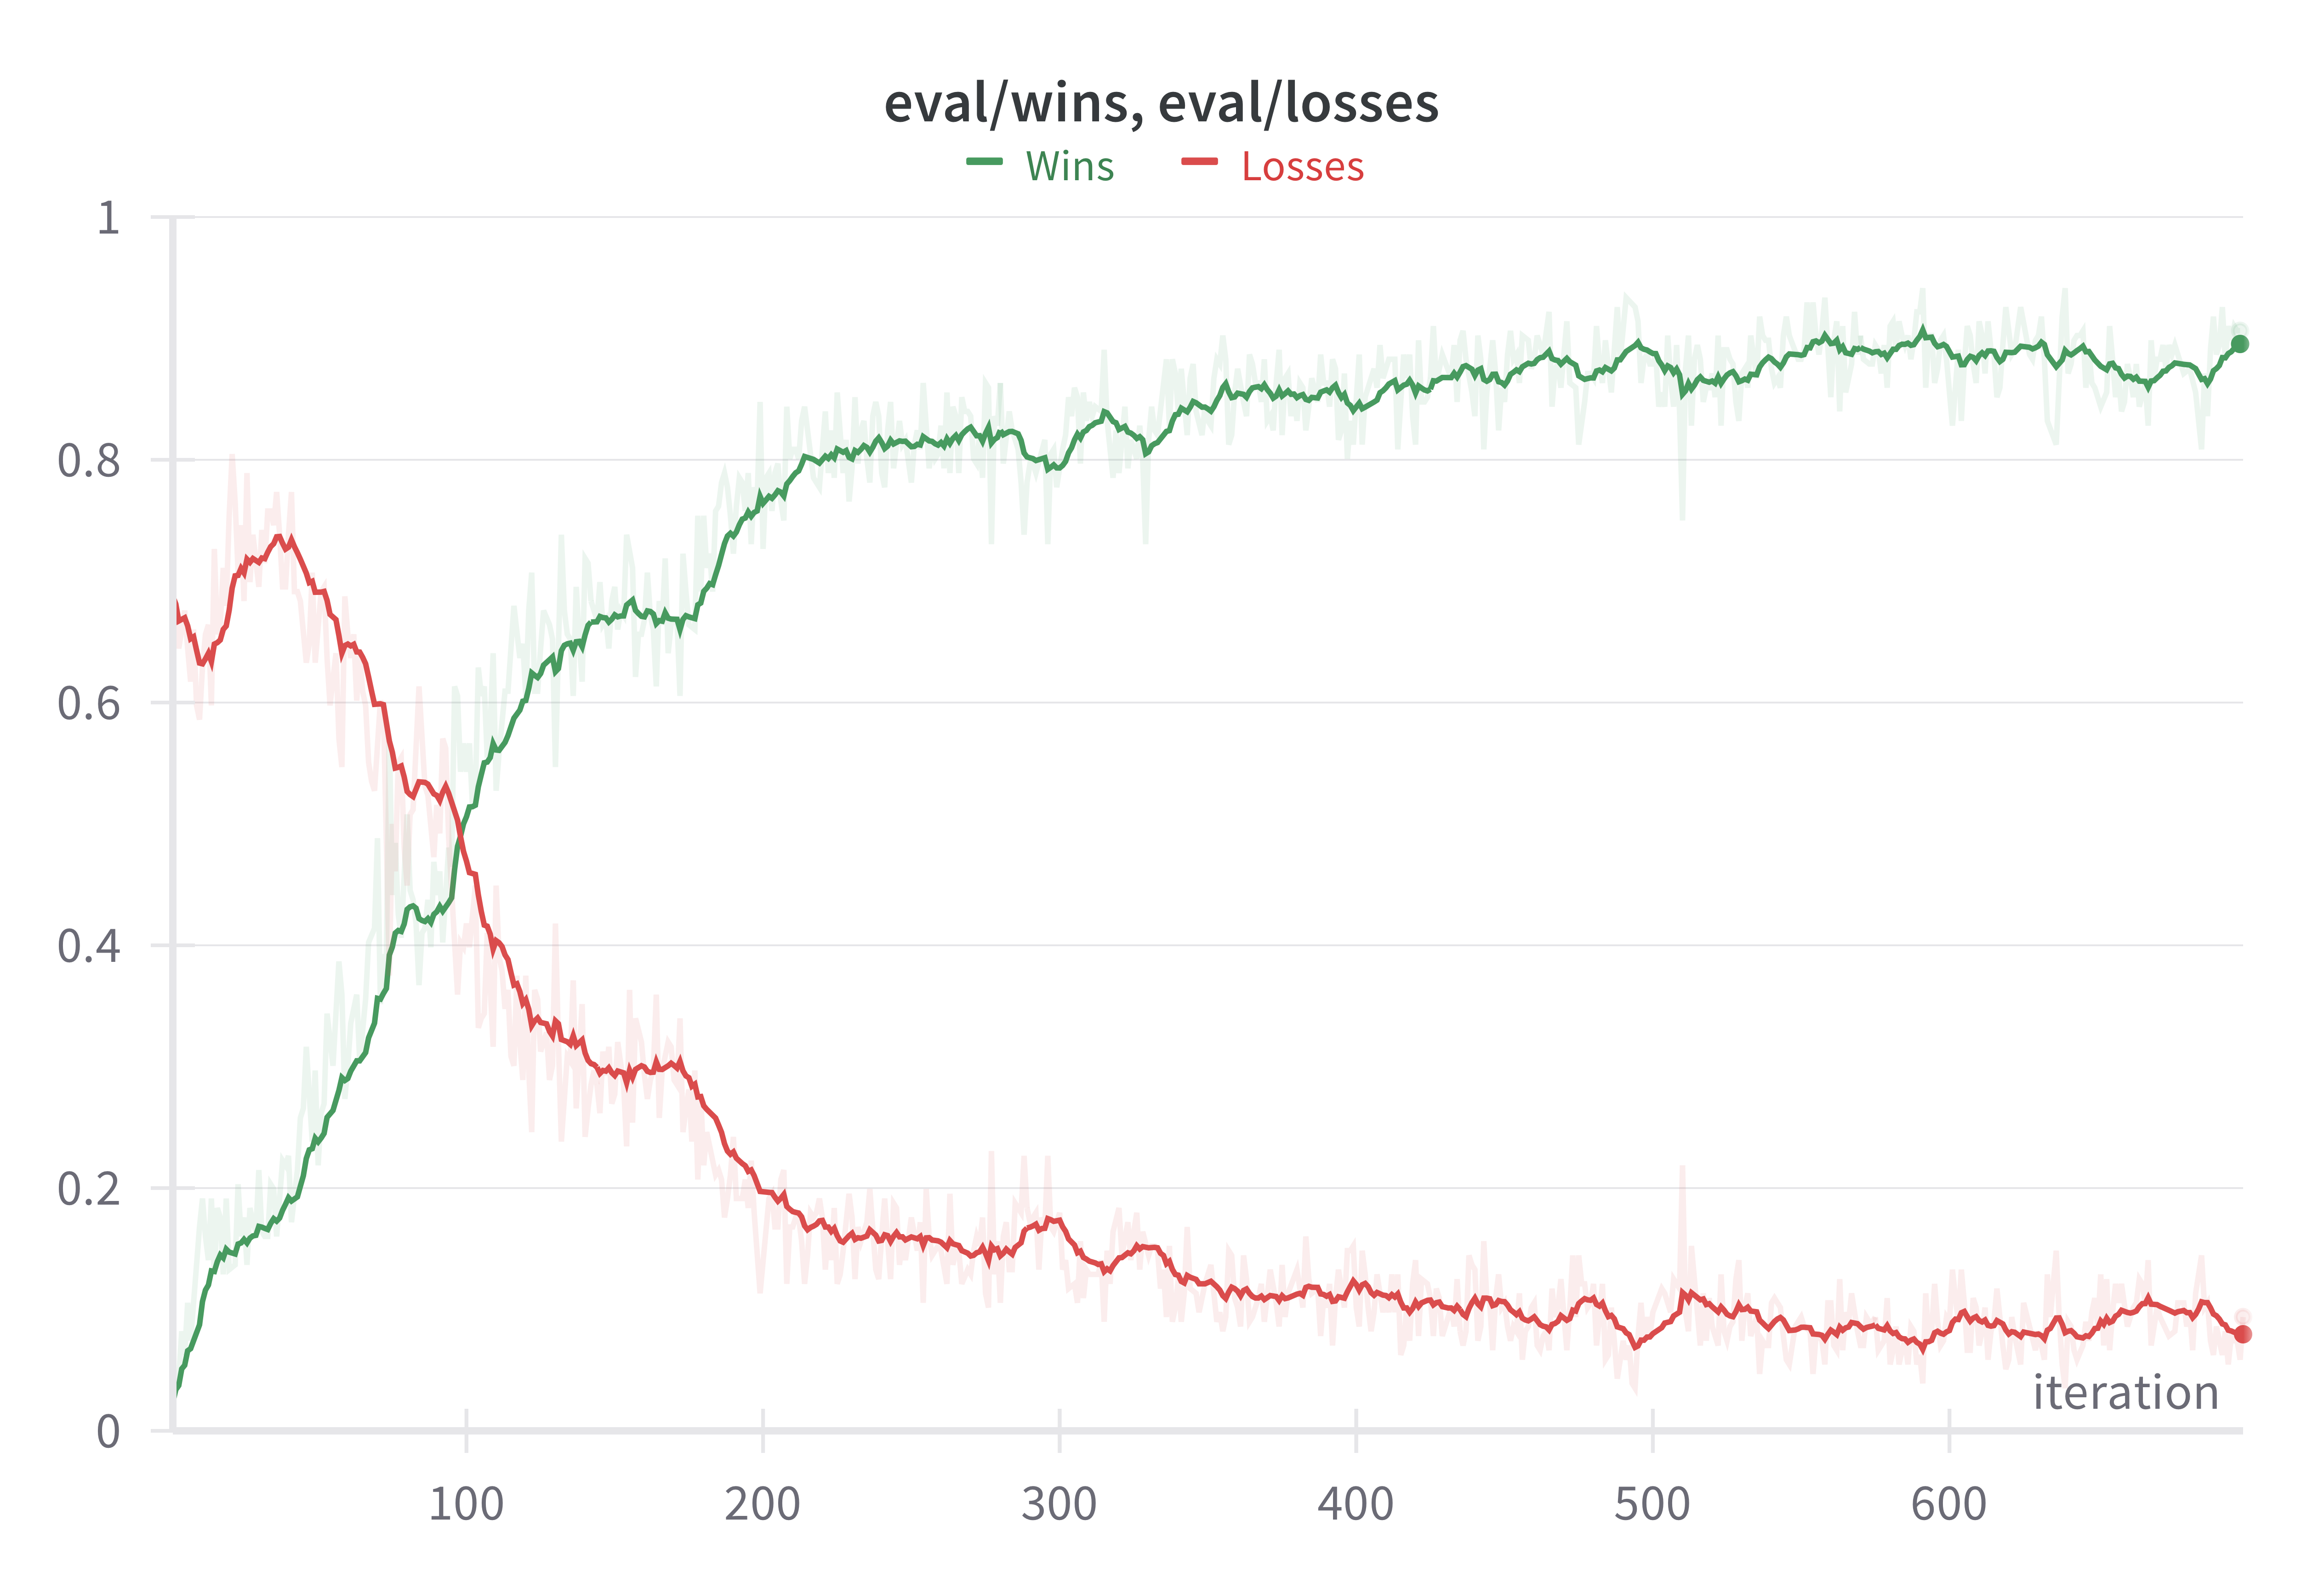
\includegraphics[width=\textwidth]{img/wykresy/othello-eval.png}
  \caption{Proces uczenia AlphaZero vs. PGX Baseline -- Othello}
  \label{fig:othello-eval}
\end{figure}

\begin{figure}[!]
  \centering
  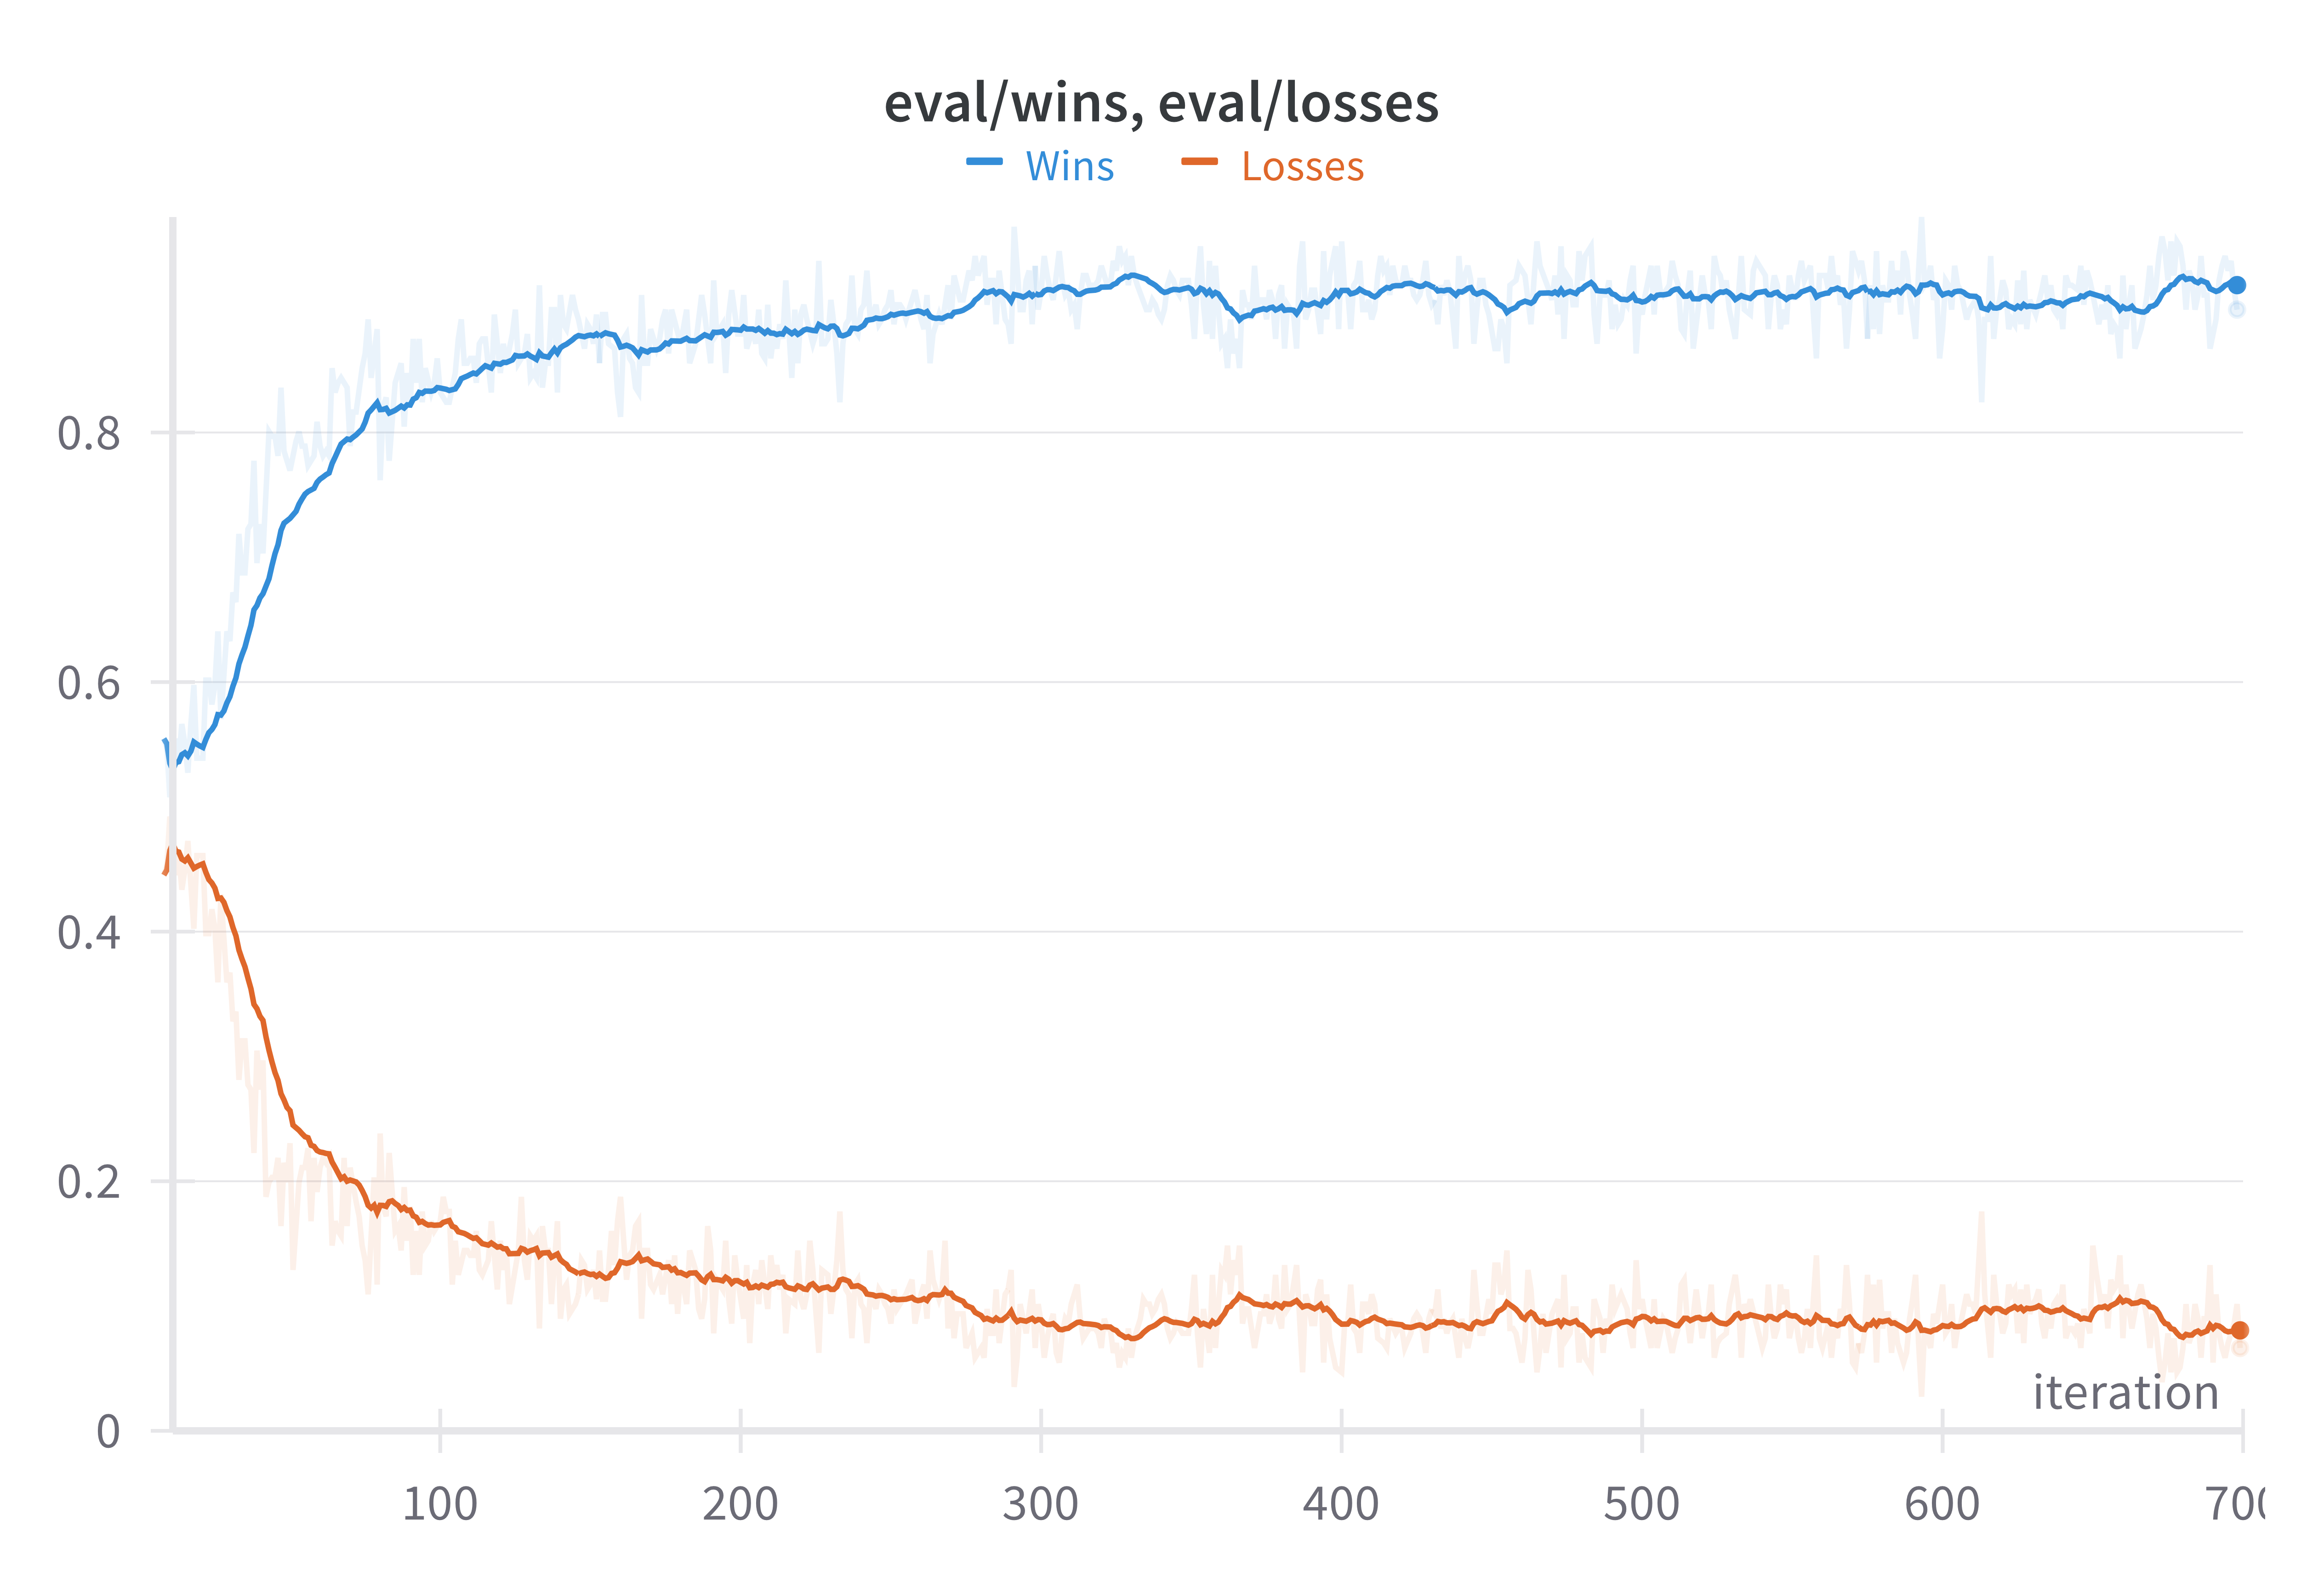
\includegraphics[width=\textwidth]{img/wykresy/bzero-eval.png}
  \caption{Proces uczenia AlphaZero vs. losowy gracz -- Brydż}
  \label{fig:bzero-eval}
\end{figure}

Ze względu na brak odpowiedniego modelu
bazowego (baseline) przeciwnika,
przeprowadzono test zaimplementowanego algorytmu
na grze Othello \cite{Othello}.
Uruchomiono identyczny proces uczenia,
wykorzystując implementację Othello oraz
model AI baseline z~\cite{PGX}.
Wyniki uczenia przedstawia Rys.~\ref{fig:othello-eval}.
Nasze AI uzyskuje stosunek wygranych do przegranych
kontra model AI baseline na poziomie 9:1.
Można zatem wnioskować, że nasza implementacja
AlphaZero jest poprawna.

\FloatBarrier

\subsection{Faza gry}

Ze względu na ograniczony czas na realizację projektu,
zdecydowano się na uproszczone podejście do fazy gry.
Zgodnie z~założeniami projektu, asystent AI powinien umożliwić
graczom doskonalenie swoich umiejętności w~grze w~brydża.
Aby zagwarantować wysoki poziom umiejętności AI, zdecydowano się
na wykorzystanie algorytmu Double Dummy Solver (DDS) \cite{DDS}.
Jest to algorytm, który wykorzystuje pełną wiedzę o~rozdaniu kart
w~celu znalezienia optymalnej sekwencji ruchów dla graczy.
Wymagane jest podanie kart wszystkich graczy, dlatego
metoda może być wykorzystana tylko przez serwer, który zna stan całej gry.
Dostosowanie poziomu trudności polega na wybieraniu nieoptymalnych ruchów
z~pewnym prawdopodobieństwem, konfigurowalnym przez użytkownika.

\section{Dodatkowe elementy aplikacji}

\subsection{Tryb mobilny}

\subsection{Motywy aplikacji}

\subsection{Grafiki wygenerowane przez AI}
